% MELON Fig. 1 — framework schematic (TikZ)
%
% Standalone build:
%   pdflatex fig_melon_framework.tex
%
% Or \input{figures/fig_melon_framework_body.tex} inside your paper,
% wrapped in a \begin{figure}...\end{figure}. The body-only version is
% the content between BEGIN BODY and END BODY below; copy it out if you
% prefer a non-standalone include.
%
% Required packages (already used in neurips_2024.tex for most):
%   tikz, xcolor, amsmath, amssymb, graphicx
% TikZ libraries: positioning, arrows.meta, calc, fit, backgrounds,
%                 shapes.geometric, decorations.pathreplacing

\documentclass[tikz,border=6pt]{standalone}
\usepackage{amsmath,amssymb}
\usepackage{xcolor}
\usepackage{graphicx}
\usetikzlibrary{positioning,arrows.meta,calc,fit,backgrounds,shapes.geometric,decorations.pathreplacing}

% ---------- palette (matches matplotlib version) ----------
\definecolor{Cmod1}{HTML}{4C78A8}   % modality 1 (blue)
\definecolor{Cmod2}{HTML}{DD8452}   % modality 2 (orange)
\definecolor{Cspat}{HTML}{5F8F71}   % spatial / GAT (green)
\definecolor{Cjoint}{HTML}{8172B2}  % joint prototype (violet)
\definecolor{Cbox}{HTML}{FAFAFA}
\definecolor{Cedge}{HTML}{1F1F1F}
\definecolor{Cmutedtext}{HTML}{666666}
\definecolor{Cfusion}{HTML}{FAFAFA}
\definecolor{Cgat}{HTML}{F7FBF8}
\definecolor{Caugblue}{HTML}{F6F8FC}
\definecolor{Caugorange}{HTML}{FCF7F1}

% ---------- BEGIN BODY ----------
\begin{document}
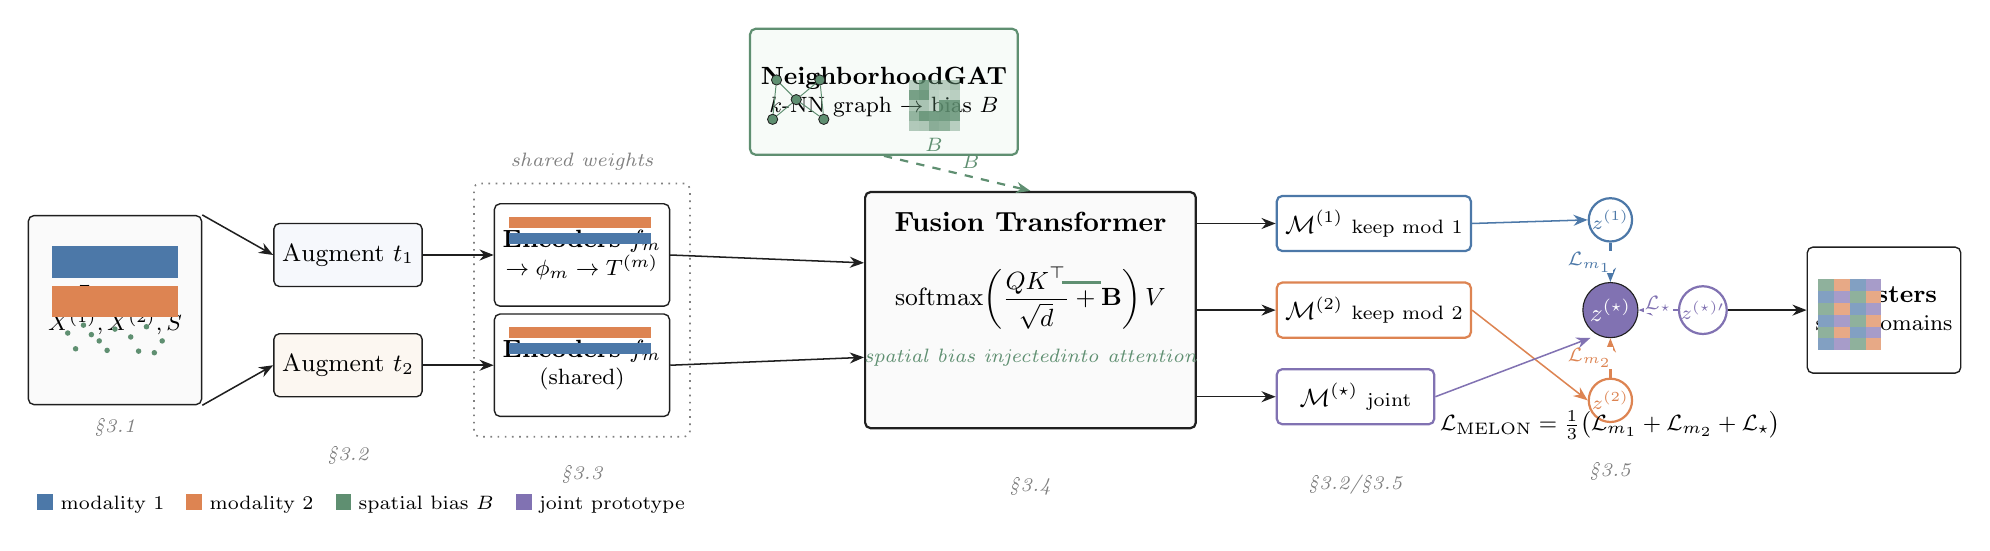
\begin{tikzpicture}[
  font=\small,
  >={Stealth[length=1.8mm,width=1.4mm]},
  stage/.style={
    draw=Cedge, rounded corners=2pt, fill=Cbox, line width=0.5pt,
    align=center, inner sep=3pt, minimum height=9mm
  },
  aug1/.style={stage, fill=Caugblue, minimum width=16mm, minimum height=8mm},
  aug2/.style={stage, fill=Caugorange, minimum width=16mm, minimum height=8mm},
  enc/.style={stage, fill=white, minimum width=22mm, minimum height=13mm},
  gat/.style={stage, draw=Cspat, fill=Cgat, line width=0.8pt,
              minimum width=34mm, minimum height=16mm},
  fusion/.style={stage, draw=Cedge, fill=Cfusion, line width=0.8pt,
                 minimum width=42mm, minimum height=30mm},
  mask/.style={stage, fill=white, minimum width=20mm, minimum height=7mm,
               line width=0.8pt},
  output/.style={stage, minimum width=12mm, minimum height=16mm, fill=white},
  flow/.style={->, draw=Cedge, line width=0.55pt},
  biasflow/.style={->, draw=Cspat, line width=0.8pt, dashed},
  pull/.style={->, line width=0.8pt},
  tag/.style={font=\scriptsize\itshape, text=gray},
]

% ===================== (1) Input =====================
\node[stage, minimum width=22mm, minimum height=24mm] (inp)
  {\textbf{Input}\\[-1pt]\footnotesize $X^{(1)}, X^{(2)}, S$};
% stacked modality heatmap thumbnails
\fill[Cmod1] ($(inp.north)+(-8mm,-4mm)$) rectangle ++(16mm,-4mm);
\fill[Cmod2] ($(inp.north)+(-8mm,-9mm)$) rectangle ++(16mm,-4mm);
% coordinate dots
\foreach \x/\y in {-6/-15, -4/-14, -2/-16, 0/-14.5, 2/-15.5, 4/-14.2,
                   6/-16, -5/-17, -1/-17.2, 3/-17.3, 5/-17.5, -3/-15.2} {
  \fill[Cspat] ($(inp.north)+(\x mm,\y mm)$) circle (0.35mm);
}
\node[tag, below=0.5mm of inp] {\S3.1};

% ===================== (2) Augmentation =====================
\node[aug1, right=9mm of inp.north east, anchor=north west, yshift=-1mm]
  (aug1) {Augment $t_1$};
\node[aug2, right=9mm of inp.south east, anchor=south west, yshift=1mm]
  (aug2) {Augment $t_2$};
\draw[flow] (inp.north east) -- (aug1.west);
\draw[flow] (inp.south east) -- (aug2.west);
\node[tag] at ($(aug1.south)!0.5!(aug2.north)$) (augtag) {};
\node[tag, below=5mm of aug2.south] {\S3.2};

% ===================== (3) Shared encoders =====================
\node[enc, right=9mm of aug1] (enc1)
  {\textbf{Encoders} $f_m$\\[-1pt]\footnotesize $\rightarrow \phi_m \rightarrow T^{(m)}$};
\node[enc, right=9mm of aug2] (enc2)
  {\textbf{Encoders} $f_m$\\[-1pt]\footnotesize (shared)};

% tiny token stripes inside encoders
\fill[Cmod1] ($(enc1.south west)+(2mm,8mm)$)  rectangle ++(18mm,1.4mm);
\fill[Cmod2] ($(enc1.south west)+(2mm,10mm)$) rectangle ++(18mm,1.4mm);
\fill[Cmod1] ($(enc2.south west)+(2mm,8mm)$)  rectangle ++(18mm,1.4mm);
\fill[Cmod2] ($(enc2.south west)+(2mm,10mm)$) rectangle ++(18mm,1.4mm);

\draw[flow] (aug1.east) -- (enc1.west);
\draw[flow] (aug2.east) -- (enc2.west);

% shared-weights dotted frame
\begin{scope}[on background layer]
  \node[draw=gray, dotted, line width=0.6pt, rounded corners=2pt,
        inner sep=2.5mm, fit=(enc1)(enc2)] (encframe) {};
\end{scope}
\node[tag, above=0.3mm of encframe.north] {shared weights};
\node[tag, below=5mm of enc2.south] {\S3.3};

% ===================== (4) NeighborhoodGAT (above main flow) =====================
\node[gat, above right=6mm and 10mm of enc1.north east] (gat)
  {\textbf{NeighborhoodGAT}\\[-1pt]\footnotesize $k$-NN graph $\rightarrow$ bias $B$};
% tiny k-NN cartoon
\begin{scope}[shift={($(gat.west)+(6mm,-1mm)$)}]
  \foreach \i/\x/\y in {0/0/0, 1/3/2.5, 2/3.5/-2.5, 3/-2.5/2.5, 4/-3/-2.5} {
  \node[circle, fill=Cspat, draw=Cedge, line width=0.3pt,
          inner sep=0pt, minimum size=1.3mm] (gn\i) at (\x mm,\y mm) {};
  }
  \foreach \a/\b in {0/1, 0/2, 0/3, 0/4, 1/2, 3/4} {
    \draw[Cspat, line width=0.35pt] (gn\a) -- (gn\b);
  }
\end{scope}
% B matrix thumbnail (5x5 greenish grid)
\begin{scope}[shift={($(gat.east)+(-14mm,-5mm)$)}]
  \foreach \i in {0,...,4} {
    \foreach \j in {0,...,4} {
      \pgfmathsetmacro{\v}{0.3+0.6*rnd}
      \fill[Cspat, opacity=\v] (\i*1.3mm,\j*1.3mm) rectangle ++(1.3mm,1.3mm);
    }
  }
  \node[font=\scriptsize\bfseries, text=Cspat] at (3.2mm,-1.8mm) {$B$};
\end{scope}

% ===================== (5) Fusion Transformer =====================
\node[fusion, right=22mm of encframe.east] (fus)
  {};
\node[font=\bfseries] at ($(fus.north)+(0,-4mm)$) {Fusion Transformer};
\node at ($(fus.center)+(0,1.5mm)$)
  {$\mathrm{softmax}\!\left(\dfrac{QK^{\top}}{\sqrt{d}} + \mathbf{B}\right) V$};
\node[font=\scriptsize\itshape, text=Cspat] at ($(fus.center)+(0,-6mm)$)
  {spatial bias injected\\into attention};
% underline the +B
\draw[Cspat, line width=1.3pt]
  ($(fus.center)+(4mm,3.5mm)$) -- ($(fus.center)+(9mm,3.5mm)$);

% encoders -> fusion
\draw[flow] (enc1.east) -- ($(fus.west)+(0,6mm)$);
\draw[flow] (enc2.east) -- ($(fus.west)+(0,-6mm)$);
% GAT B -> fusion (dashed green)
\draw[biasflow] (gat.south) -- node[above right=-1mm, font=\scriptsize\bfseries,
                                     text=Cspat] {$B$}
                ($(fus.north)+(0,0)$);
\node[tag, below=5mm of fus.south] {\S3.4};

% ===================== (6) Masked views =====================
\node[mask, draw=Cmod1, right=10mm of fus.east, yshift=11mm] (m1)
  {$\mathcal{M}^{(1)}$ \scriptsize keep mod 1};
\node[mask, draw=Cmod2, right=10mm of fus.east] (m2)
  {$\mathcal{M}^{(2)}$ \scriptsize keep mod 2};
\node[mask, draw=Cjoint, right=10mm of fus.east, yshift=-11mm] (ms)
  {$\mathcal{M}^{(\star)}$ \scriptsize joint};

\draw[flow] (fus.east |- m1.west) -- (m1.west);
\draw[flow] (fus.east |- m2.west) -- (m2.west);
\draw[flow] (fus.east |- ms.west) -- (ms.west);
\node[tag, below=5mm of ms.south] {\S3.2/\S3.5};

% ===================== (7) PID contrastive loss =====================
% joint prototype (center)
\node[circle, fill=Cjoint, draw=Cedge, line width=0.4pt,
      minimum size=7mm, inner sep=0pt,
      right=14mm of m2] (zstar) {\color{white}\small\bfseries $z^{(\star)}$};

% satellites
\node[circle, draw=Cmod1, line width=0.8pt, fill=white,
      minimum size=5.5mm, inner sep=0pt,
      above=5mm of zstar] (z1)
      {\color{Cmod1}\scriptsize\bfseries $z^{(1)}$};
\node[circle, draw=Cmod2, line width=0.8pt, fill=white,
      minimum size=5.5mm, inner sep=0pt,
      below=5mm of zstar] (z2)
      {\color{Cmod2}\scriptsize\bfseries $z^{(2)}$};
\node[circle, draw=Cjoint, line width=0.8pt, fill=white,
      minimum size=5.5mm, inner sep=0pt,
      right=5mm of zstar] (zsp)
      {\color{Cjoint}\scriptsize\bfseries $z^{(\star)\prime}$};

\draw[pull, Cmod1]  (z1)  -- node[midway, left=-0.5mm,
                                 font=\scriptsize\bfseries, text=Cmod1,
                                 fill=white, inner sep=0.4pt] {$\mathcal{L}_{m_1}$} (zstar);
\draw[pull, Cmod2]  (z2)  -- node[midway, left=-0.5mm,
                                 font=\scriptsize\bfseries, text=Cmod2,
                                 fill=white, inner sep=0.4pt] {$\mathcal{L}_{m_2}$} (zstar);
\draw[pull, Cjoint] (zsp) -- node[midway, above=-0.5mm,
                                 font=\scriptsize\bfseries, text=Cjoint,
                                 fill=white, inner sep=0.4pt] {$\mathcal{L}_{\star}$} (zstar);

% mask -> satellite feeders
\draw[flow, Cmod1]  (m1.east) -- (z1.west);
\draw[flow, Cmod2]  (m2.east) -- (z2.west);
\draw[flow, Cjoint] (ms.east) -- ([yshift=-1mm]zstar.south west);

% total loss
\node[below=8mm of zstar, font=\footnotesize] (totloss)
  {$\mathcal{L}_{\mathrm{MELON}}
    = \tfrac{1}{3}\bigl(\mathcal{L}_{m_1}+\mathcal{L}_{m_2}+\mathcal{L}_{\star}\bigr)$};
\node[tag, below=0.5mm of totloss] {\S3.5};

% ===================== (8) Output =====================
\node[output, right=10mm of zsp] (clust) {\textbf{Clusters}\\[-1pt]\footnotesize spot domains};
% mock cluster grid
\foreach \i in {0,...,3} {
  \foreach \j in {0,...,5} {
    \pgfmathtruncatemacro{\c}{mod(\i*3+\j*2,4)}
    \ifcase\c
      \fill[Cmod1!70]  ($(clust.south west)+(1.5mm+\i*2mm, 3mm+\j*1.5mm)$)
                      rectangle ++(2mm,1.5mm);
    \or
      \fill[Cmod2!70]  ($(clust.south west)+(1.5mm+\i*2mm, 3mm+\j*1.5mm)$)
                      rectangle ++(2mm,1.5mm);
    \or
      \fill[Cspat!70]  ($(clust.south west)+(1.5mm+\i*2mm, 3mm+\j*1.5mm)$)
                      rectangle ++(2mm,1.5mm);
    \or
      \fill[Cjoint!70] ($(clust.south west)+(1.5mm+\i*2mm, 3mm+\j*1.5mm)$)
                      rectangle ++(2mm,1.5mm);
    \fi
  }
}
\draw[flow] (zsp.east) -- (clust.west);

% ===================== Legend =====================
\node[below=10mm of inp.south west, anchor=north west,
      font=\scriptsize] (leg) {%
  \tikz\fill[Cmod1]  (0,0) rectangle (2mm,2mm);~modality 1\quad
  \tikz\fill[Cmod2]  (0,0) rectangle (2mm,2mm);~modality 2\quad
  \tikz\fill[Cspat]  (0,0) rectangle (2mm,2mm);~spatial bias $B$\quad
  \tikz\fill[Cjoint] (0,0) rectangle (2mm,2mm);~joint prototype
};

\end{tikzpicture}
\end{document}
% ---------- END BODY ----------
